\vfill 
\chapter{Fondements de l'Intelligence Artificielle et de l'Infrastructure Cloud dans notre Plateforme}
\label{chap:fondements de l'Intelligence Artificielle et de l'Infrastructure Cloud dans notre Plateforme}
\mtcaddchapter
\section*{Introduction}
\justifying
Ce chapitre explore les fondements de l'Intelligence Artificielle (IA) et de l'infrastructure cloud dans notre plateforme. Nous aborderons des définitions et explications des concepts clés de l’AI et de l’apprentissage profond, notre choix de l'algorithme MoE et l'intégration du cloud. Cette compréhension nous permettra de saisir les capacités de notre plateforme.

\section{L'intelligence artificielle dans notre plateforme}
\justifying
Cette section sera consacrée à la présentation des concepts de base sur 
l’intelligence artificielle.
\subsection{Définitions}
\justifying
Dans cette partie, nous allons définir l'intelligence artificielle et l'apprentissage profond.


\subsubsection{Intelligence artificielle}
\justifying
L'intelligence artificielle concerne la création de machines capables de penser et d'agir comme des êtres humains \cite{ai}. En d'autres termes, c'est la science qui vise à créer des programmes informatiques et des machines qui peuvent imiter le raisonnement humain, apprendre de l'expérience et accomplir des tâches variées de manière autonome.

\subsubsection{Apprentissage profond}
\justifying
L'apprentissage profond, connu sous le nom de deep learning, est une branche de l’IA qui se concentre sur l'entraînement de réseaux de neurones artificiels \cite{deepLearning}.\\
Ces réseaux de neurones sont organisés en couches. Chaque couche transforme l'entrée qu'elle reçoit pour produire une sortie. Ces transformations sont ajustées automatiquement pendant l'apprentissage pour améliorer les performances du système.

\subsection{Explication des concepts clés}
\justifying
Dans cette section, nous allons clarifier quelques concepts fondamentaux.

\subsubsection{Natural Language Model (NLP)}
\justifying
Les modèles de langage naturel (NLP) sont des composants de l'intelligence artificielle conçus pour comprendre et générer un langage humain naturel. Ils sont largement utilisés dans des applications telles que la traduction automatique, la génération de texte et l'analyse du sentiment. Ces modèles sont entraînés sur de grandes quantités de données textuelles afin d'apprendre les structures linguistiques et de capturer les nuances du langage.

\subsubsection{Large Model Language (LLM)}
\justifying
Les modèles de langage de grande taille (LLM) sont des modèles d'intelligence artificielle qui ont été entraînés sur de vastes ensembles de données textuelles pour acquérir une compréhension approfondie du langage naturel. Ces modèles sont capables de générer du texte cohérent et de qualité et sont souvent utilisés pour une variété de tâches en NLP.

\subsubsection{Tokenizers  }
\justifying
Les tokenizers sont des outils essentiels en traitement automatique du NLP qui découpent le texte en unités plus petites appelées "tokens". Ces tokens peuvent être des mots, des sous-mots ou même des caractères individuels. Ils servent de points de départ pour l'analyse et le traitement du texte.

\subsubsection{Retrieval Augmented Generation (RAG) }
RAG est un concept utilisé dans le domaine de l'intelligence artificielle et le traitement du langage naturel. Il utilise des techniques de récupération d'informations pour améliorer la génération de texte par des modèles de langage. \\
En d'autres termes, au lieu de simplement générer du texte en fonction de ce que le modèle a appris pendant son entraînement, un système RAG va d'abord chercher dans une grande base de données de textes pour trouver des informations pertinentes. Il utilisera ensuite ces informations pour générer une réponse plus informée et précise.\\
Notons que cette base de données de textes peut être vectorielle. C'est-à-dire que les textes sont représentés sous forme de vecteurs dans un espace vectoriel. Ceci permet de les comparer et de les rechercher de manière efficace.

\subsubsection{Dynamic Retrieval Augmented Generation (Dynamic RAG)}
\justifying
Dynamic RAG (Retrieval Augmented Generation) est une approche avancée de RAG qui permet d'adapter dynamiquement la récupération d'informations en fonction du contexte de la requête de l'utilisateur.\\
Dans un système RAG standard, la stratégie de récupération d'informations est généralement fixe et déterminée à l'avance. Par exemple, le système doit toujours chercher dans la même base de données de textes.\\
Alors que dans un système Dynamic RAG, le système peut adapter sa stratégie de récupération d'informations en fonction de la tâche à accomplir. Par exemple, pour une tâche de réponse à des questions, le système peut chercher dans une base de données de textes spécifique.\\
Cette approche permet au système d'être plus flexible et adaptable, ce qui lui permet d’améliorer ses performances sur une variété de tâches.\\
La Figure 2.1. synthétise les étapes et le déroulement  de Dynamic RAG.

\begin{figure}[H]
    \centering
    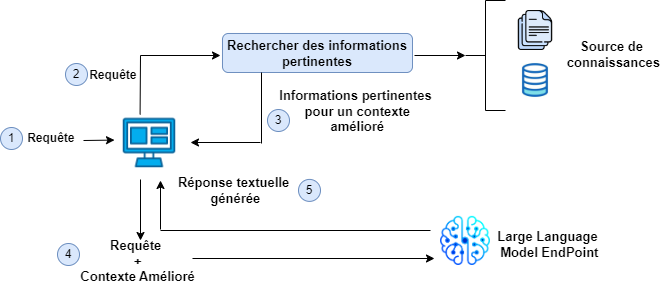
\includegraphics[width=\textwidth]{images/chp2/fig1.png}
   \caption{Le déroulement et les étapes de Dynamic RAG}
    \label{fig:deroulement dynamic rag}      
\end{figure}


\subsection{Algorithme d’Apprentissage Adopté}
\justifying
Dans cette section, nous expliquerons le Sparse Mixture of Experts (MoE), l’algorithme d’apprentissage adopté. Nous aborderons l'introduction à cet algorithme, la définition de la couche Sparse MoE et son architecture ainsi que le processus de formation et d'inférence associé.\\
Bien notez que les informations de cette section sont issues de la référence suivante. \cite{moe}

\subsubsection{Couche Sparse MoE et son architecture}
\justifying
La couche Sparse MoE est une composante clé des modèles de transformers remplaçant les couches traditionnelles de réseaux de neurones denses. Chaque couche Sparse MoE est constituée de multiples "experts" qui sont essentiellement des réseaux de neurones. Ces experts sont souvent des réseaux feed-forward (FFN) et peuvent aussi être plus complexes ou former un autre MoE permettant ainsi des MoEs hiérarchiques.\\
En plus des experts, une couche Sparse MoE inclut un réseau de portes ou "routeur". Ce routeur détermine comment les tokens sont distribués aux experts. Il est important de noter qu'un même token peut être attribué à plusieurs experts.\\
Le routeur est constitué de paramètres appris et entraîné avec le reste du réseau.\\
La Figure 2.2. synthétise l’architecture de l’algorithme Sparse Mixture of Experts.

\begin{figure}[H]
    \centering
    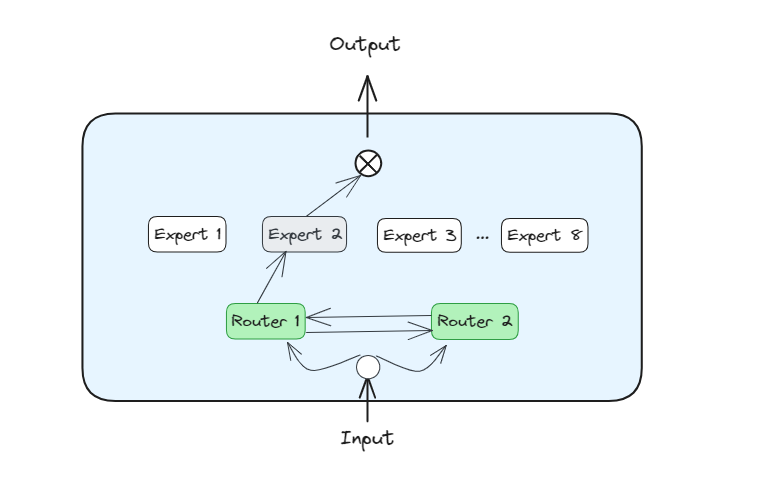
\includegraphics[width=\textwidth]{images/chp2/fig2.png}
    \caption{Le déroulement de l’algorithme Sparse Mixture of Experts}
    \label{fig:architecture sparse moe}    
\end{figure}

\subsubsection{ Fonctionnement de l'algorithme Sparse Mixture of Experts}
\justifying
L'algorithme sparse Mixture of Experts est une méthode avancée qui combine les avantages des modèles experts spécialisés avec la flexibilité des modèles généralistes.\\
Contrairement aux réseaux neuronaux traditionnels qui utilisent une seule architecture de modèle pour traiter toutes les entrées, le MoE divise le processus d'apprentissage en plusieurs experts spécialisés. Ces experts sont ensuite combinés de manière pondérée pour générer une prédiction finale (voir Figure 2.2). Chaque expert est responsable de traiter une portion spécifique de l'entrée en apportant ainsi sa propre expertise à la résolution du problème. Ces experts peuvent être considérés comme des sous-modèles qui se spécialisent dans différentes parties de l'espace d'entrée.\\
L'approche sparse du MoE signifie que seuls quelques experts sont activés pour chaque exemple d'entrée. Elle permet une utilisation efficace des ressources computationnelles et une adaptation dynamique aux différentes conditions d'entrée. Cette activation sélective des experts est déterminée par des routeurs qui dirigent l'entrée vers les experts les plus pertinents en fonction de son contenu.

\subsubsection{Processus de formation et d'inférence}
\justifying
Le processus d'entraînement de Mixture of Experts (MoE) implique simultanément l'apprentissage des paramètres des experts et du routeur. \\
Pendant la formation, chaque jeton d'entrée est dirigé vers un ou plusieurs experts en fonction des poids appris par le routeur. Les experts traitent ces jetons et retournent leurs sorties respectives. Ces sorties sont combinées pour former la sortie finale du MoE utilisée pour calculer la perte et mettre à jour les paramètres du modèle.
En phase d'inférence, seuls les experts les plus pertinents sont sélectionnés selon les poids du routeur en réduisant ainsi la complexité de calcul et améliorant l'efficacité du MoE. Bien que tous les paramètres doivent être chargés en mémoire, seuls ceux nécessaires sont utilisés pendant l'inférence.

\subsubsection{Raisons du Choix de l'Algorithme Sparse Mixture of Experts }
\justifying
Le choix d'adopter l'algorithme Sparse Mixture of Experts (MoE) repose sur sa capacité à optimiser l'utilisation des ressources computationnelles en ne faisant fonctionner que les parties pertinentes du modèle. Cela permet d'augmenter l'efficacité de l'apprentissage et réduire la charge de calcul qui est essentiel pour des applications à grande échelle nécessitant des modèles complexes.\\
En intégrant le Sparse MoE dans notre plateforme, nous sommes en mesure de fournir des réponses plus précises et adaptées aux besoins spécifiques de chaque utilisateur en améliorant ainsi l'expérience globale d'apprentissage.


\section{Le Cloud dans notre plateforme}
\justifying
Dans cette partie, nous allons présenter le cloud computing, les types de cloud ainsi que le type de cloud adopté dans notre plateforme.

\subsection{Présentation du cloud computing}
\justifying
Le cloud computing est une technologie qui permet d'accéder à des ressources informatiques en utilisant l’internet.\\
L'infrastructure cloud joue un rôle crucial dans le bon fonctionnement et l'évolutivité de notre application. Elle nous permet de bénéficier de services performants et sécurisés en optimisant nos coûts d'exploitation.

\subsection{Type de cloud}
\justifying
Dans cette section, nous présenterons les types de cloud, suivi par le type adopté.

\subsubsection{Types d'infrastructures de cloud computing}
\justifying
Le cloud computing est divisé en trois types principaux : public, privé et hybride.
\begin{itemize}[itemsep=2pt, parsep=2pt]
    \item \textbf{Cloud privé}\\ Un cloud privé est un environnement de cloud computing dédié à une seule organisation.Dans un cloud privé, toutes les ressources sont isolées et sous le contrôle d'une seule organisation. Ainsi, le cloud privé est également appelé cloud interne ou d'entreprise. \cite{cloudPrivé}
    \item \textbf{Cloud publique}\\ Un cloud public est une infrastructure informatique dans laquelle un fournisseur de services met des ressources à la disposition du public via internet. Les ressources varient selon le fournisseur mais peuvent inclure des capacités de stockage, des applications ou des machines virtuelles. \cite{CloudPublique}
    \item \textbf{Cloud hybride}\\ Un cloud hybride est un environnement informatique mixte dans lequel des applications s'exécutent à l'aide d'une combinaison de ressources de calcul, de stockage et de services dans différents environnements (clouds publics et clouds privés, y compris des centres de données sur site ou en périphérie). \cite{CloudHybride}
\end{itemize}

\subsubsection{Type de cloud adopté }
\justifying
Notre application repose sur une architecture Cloud hybride qui combine à la fois des services de Cloud public et de Cloud privé. Cette approche nous permet de tirer parti des avantages de chaque modèle en fonction des besoins spécifiques de notre application. 

\subsection{Avantages de l’adoption du cloud dans notre projet}
\justifying
L'infrastructure Cloud offre de nombreux avantages pour notre projet. Tout d'abord, elle nous permet de bénéficier d'une grande scalabilité en adaptant automatiquement les ressources allouées en fonction des besoins de notre application. De plus, elle garantit une haute disponibilité et une redondance des données grâce à la répartition géographique des serveurs. Enfin, l'infrastructure Cloud nous permet de réduire nos coûts d'exploitation. 

\subsection{Service cloud adoptés }
\justifying
Parmi les services Cloud intégrés dans notre plateforme, nous retrouvons le Runtime Edge, le Serverless et le \textbf{CDN} (\textbf{C}ontent \textbf{D}elivery \textbf{N}etwork).\\
Les services cloud utilisés dans notre plateforme sont présentés dans le tableau 2.1.


\begin{table}[H]
    \centering
    \caption{Descriptions des services de cloud computing}
    \begin{tabular}{|>{\RaggedRight\arraybackslash}p{4cm}|>{\RaggedRight\arraybackslash}p{10cm}|}
        \hline
        \textbf{Service} & \textbf{Description} \\
        \hline
        \textbf{Runtime Edge} & Edge Runtime est idéal pour la diffusion de contenu dynamique et personnalisé avec une faible latence en utilisant de petites fonctions simples. Sa rapidité provient de l'utilisation minimale des ressources, mais cela peut être limité dans de nombreux scénarios. Dans notre application, Edge Runtime est utilisé pour optimiser la diffusion de contenu personnalisé pour garantir ainsi une expérience utilisateur rapide et réactive. \\
        \hline
        \textbf{Serverless} & Les architectures sans serveur, ou Serverless, permettent de déléguer la gestion des serveurs à un fournisseur de services Cloud. Cette approche offre plusieurs avantages tels qu'une réduction des coûts d'exploitation, une scalabilité automatique et une simplification de la maintenance. Dans notre application, le Serverless est utilisé pour gérer les fonctions backend telles que le traitement des données et la gestion des Application Programming Interface (API). \\
        \hline
        \textbf{Content Delivery Network} & Un Content Delivery Network (CDN) est un réseau de serveurs distribués géographiquement qui permet de distribuer du contenu à grande échelle. L'utilisation d'un CDN permet d'améliorer les performances de notre application en réduisant la latence et en optimisant la bande passante. Dans notre cas, le CDN est utilisé pour distribuer les ressources statiques de notre application telles que les images, les feuilles de style et les scripts. \\
        \hline
    \end{tabular}
    \label{table:cloud_services}
\end{table}

\section*{Conclusion}
\justifying
Notre application exploite des techniques d'apprentissage profond et une infrastructure cloud avancée pour offrir une expérience utilisateur optimale et répondre aux exigences de performance et de fiabilité. Le chapitre suivant approfondira les exigences fonctionnelles et non fonctionnelles pour concevoir notre solution adaptée.


